% TODO:
% - 

%%%%%%%%%%%%%%%%%%%%%%%%%%%%%%%%%%%%%%%%%%%%%%%%%%%%
% documentclss
\documentclass[]{beamer}
%\documentclass[handout]{beamer} %Drucker Version


%%%%%%%%%%%%%%%%%%%%%%%%%%%%%%%%%%%%%%%%%%%%%%%%%%%%
% packages

\usepackage[utf8]{inputenc}
\usepackage[ngerman]{babel}
\usepackage[T1]{fontenc}

\usepackage{setspace}
\usepackage{microtype}
\usepackage{lmodern}

\usepackage{graphicx}
\graphicspath{{images/}}

\hypersetup{
  pdftex,
  bookmarks, bookmarksopen, bookmarksopenlevel=1, bookmarksnumbered=true,
  pdfpagemode={UseNone},
  pdfpagelayout={SinglePage},
  plainpages=false,
  pdfkeywords={Robuste Systeme, ISO 26262},
  pdfsubject={Robuste Systeme - ISO 26262},
  pdftitle={Robuste Systeme - ISO 26262},
  pdfauthor={Martin Wichmann}
}

\usepackage{booktabs}
\usepackage{multirow}


\newtranslation[to=ngerman]{Example}{Beispiel}


\usetheme{Warsaw}



\AtBeginSection[]
{
   \begin{frame}
        \frametitle{Inhaltsübersicht}
        \tableofcontents[currentsection,currentsubsection]
   \end{frame}
}



%%%%%%%%%%%%%%%%%%%%%%%%%%%%%%%%%%%%%%%%%%%%%%%%%%%%
% Title
\author{Martin Wichmann}
\title{ISO 26262}
\date{\today}
\institute{Ostfalia Hochschule für angewandte Wissenschaften}




%%%%%%%%%%%%%%%%%%%%%%%%%%%%%%%%%%%%%%%%%%%%%%%%%%%%
% begin document
\begin{document}

\begin{frame}
\maketitle
\end{frame}


\begin{frame}
\frametitle{Inhaltsübersicht}
\tableofcontents
\end{frame}





%%%%%%%%%%%%%%%%%%%%%%%%%%%%%%%%%%%%%%%%%%%%%%%%%%%%%%%%%%%%%%%%%%%5
% Einleitung
\section{Einleitung}
\label{sec:einleitung}

\begin{frame}
\frametitle{Information zu Ausarbeitung und Präsentation}
\begin{itemize}
    \item ISO Norm nicht verfügbar
    \item Kaum Literatur vorhanden
    \item Ausarbeitung und Präsentation basieren fast komplett auf \cite{1}
    \begin{itemize}
        \item Befasst sich vor allem mit DIN 61508
    \end{itemize}
    \item Bilder sind aus Buch übernommen
\end{itemize}
\end{frame}


\begin{frame}
\frametitle{Funktionale Sicherheit}

\begin{itemize}
    \item Methodischer Ansatz für Sicherheit
    \item Beschreibt feste Anforderungen und Vorgehensweisen
    \item Sicherheit soll möglichst Objektiv werden
    \item Funktionale Sicherheit lediglich allgemeines Konzept
    \item Implementationen zum Beispiel:
    \begin{itemize}
        \item DIN 61508 (E/E/PES)
        \item ISO 26262 (Personenkraftwagen)
        \item DIN 60601 (Medizin-Geräte)
    \end{itemize}
\end{itemize}

\end{frame}


\begin{frame}
\frametitle{ISO 26262}

\begin{itemize}
    \item Internationale Norm für Automotive-Bereich
    \item Freigabe: 14. November 2011
    \item Kapitel 10 fehlt noch
    \item Basiert auf DIN 61508 (1998) und erweitert diese
    \begin{itemize}
        \item Serienproduktion
        \item Wartung
        \item Außerbetriebnahme
    \end{itemize}
\end{itemize}

\end{frame}




\begin{frame}
\frametitle{Struktur ISO 26262}

\begin{enumerate}
    \item Vokabular
    \item Management der funktionalen Sicherheit
    \item Konzept-Phase
    \item Produktentwicklung: Systemebene
    \item Produktentwicklung: Hardwareebene
    \item Produktentwicklung: Softwareebene
    \item Produktion, Betrieb und Außerbetriebnahme
    \item Unterstützende Prozesse
    \item ASIL- und sicherheitsorientierte Analysen
    \item Guideline
\end{enumerate}

\end{frame}



%%%%%%%%%%%%%%%%%%%%%%%%%%%%%%%%%%%%%%%%%%%%%%%%%%%%%%%%%%%%%%%%%%%5
% Sicherheitslebenszyklus und Planung
\section{Sicherheitslebenszyklus und Planung}
\label{sec:Sicherheitslebenszyklus_Planung}

\begin{frame}
\frametitle{Überblick Sicherheitslebenszyklus}
\begin{figure}
   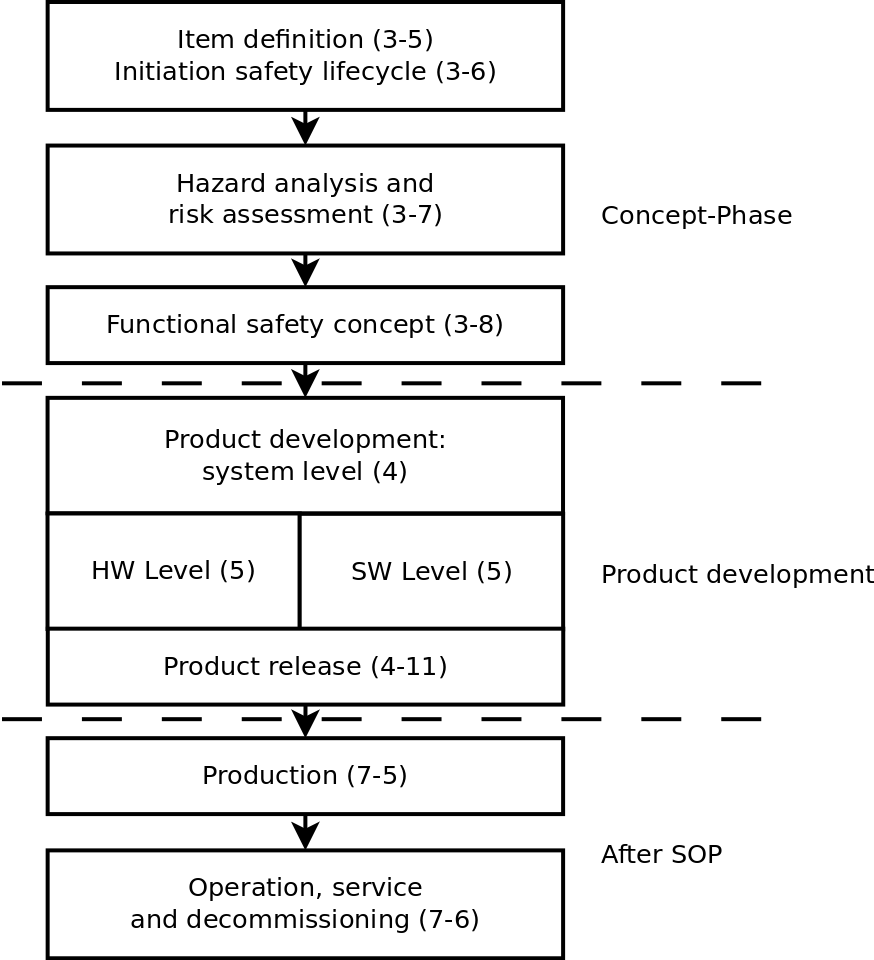
\includegraphics[width=6cm]{Abb_6_1}
\end{figure}
\end{frame}


\begin{frame}
\frametitle{Management der funktionalen Sicherheit}

\begin{itemize}
    \item Genaue Dokumentation der Sicherheit und des Projektes
    \item Geforderte Dokumente (Auszug):
    \begin{itemize}
        \item Ausbildungs- und Qualifizierungsnachweise
        \item Sicherheitsplan
        \item Review-, Audit- und Assessmentplan
        \item Sicherheitsnachweise
    \end{itemize}
    \item Dokumentation\dots
    \begin{itemize}
        \item \dots während des gesamten Projektes
        \item \dots ausführlich (Wer, Wann, Was, Warum)
        \item \dots Nachvollziehbar und Nicht-Abstreitbar
    \end{itemize}
\end{itemize}

\end{frame}

\begin{frame}
\frametitle{Gefährdungsanalyse und Risikoeinschätzung I}

\begin{itemize}
    \item Ermitteln aller relevanten Fahrzeugzustände und Fahrsituationen
    \item Ermitteln möglicher funktionaler Fehler
    \item Bewerten der Risiken jeder Gefährdungssituation in allen Fahrsituationen
    \item Festlegen der notwendigen Risikominderung (ASIL)
    \item Ableiten der Sicherheitsziele
\end{itemize}

\end{frame}


\begin{frame}
\frametitle{Gefährdungsanalyse und Risikoeinschätzung II}

\begin{itemize}
    \item Häufigkeit der Fahrsituation (Exposure E)
    \begin{itemize}
        \item E0 bis E4
    \end{itemize}
    \item Schwere eines möglichen Schadens (Severity S)
    \begin{itemize}
        \item S0 bis S3
    \end{itemize}
    \item Beherrschbarkeit durch den Fahrer (Controllability C)
    \begin{itemize}
        \item C0 bis C3
    \end{itemize}
\end{itemize}

\end{frame}


\begin{frame}
\frametitle{Gefährdungsanalyse und Risikoeinschätzung III}

\center
{
\small
\begin{tabular}[h]{c c | c c c}

\toprule
 &  & C1 & C2 & C3\\
\midrule
\multirow{4}{*}{S1} & E1 & QM & QM & QM\\
 & E2 & QM & QM & QM\\
 & E3 & QM & QM & ASIL A\\
 & E4 & QM & ASIL A & ASIL B\\
\midrule
\multirow{4}{*}{S2} & E1 & QM & QM & QM\\
 & E2 & QM & QM & ASIL A\\
 & E3 & QM & ASIL A & ASIL B\\
 & E4 & ASIL A & ASIL B & ASIL C\\
\midrule
\multirow{4}{*}{S3} & E1 & QM & QM & ASIL A\\
 & E2 & QM & ASIL A & ASIL B\\
 & E3 & ASIL A & ASIL B & ASIL C\\
 & E4 & ASIL B & ASIL C & ASIL D\\
\bottomrule
\end{tabular}
}

\end{frame}




\begin{frame}
\frametitle{Gefährdungsanalyse und Risikoeinschätzung III}

\begin{example}[Analyse einer Servolenkung]
    \begin{itemize}
    \item Bei einer Stadtfahrt (etwa 50 km/h) kommt es zu unmotivierten Lenkbewegungen
        \begin{itemize}
            \item E = E4
            \item C = C3
            \item S = S2
            \item ASIL C
        \end{itemize}
    \item Selbe Situation bei einer Landstraßenfahrt (etwa 100 km/h)
        \begin{itemize}
            \item E = E4
            \item C = C3
            \item S = S3
            \item ASIL D
        \end{itemize}
    \item Servolenkung: ASIL D
    \end{itemize}
\end{example}


\end{frame}


%%%%%%%%%%%%%%%%%%%%%%%%%%%%%%%%%%%%%%%%%%%%%%%%%%%%%%%%%%%%%%%%%%%5
% Produktentwicklung
\section{Produktentwicklung}
\label{sec:Produktentwicklung}

\subsection{Systemebene}
\begin{frame}
\frametitle{Systemebene Überblick}

\begin{figure}
   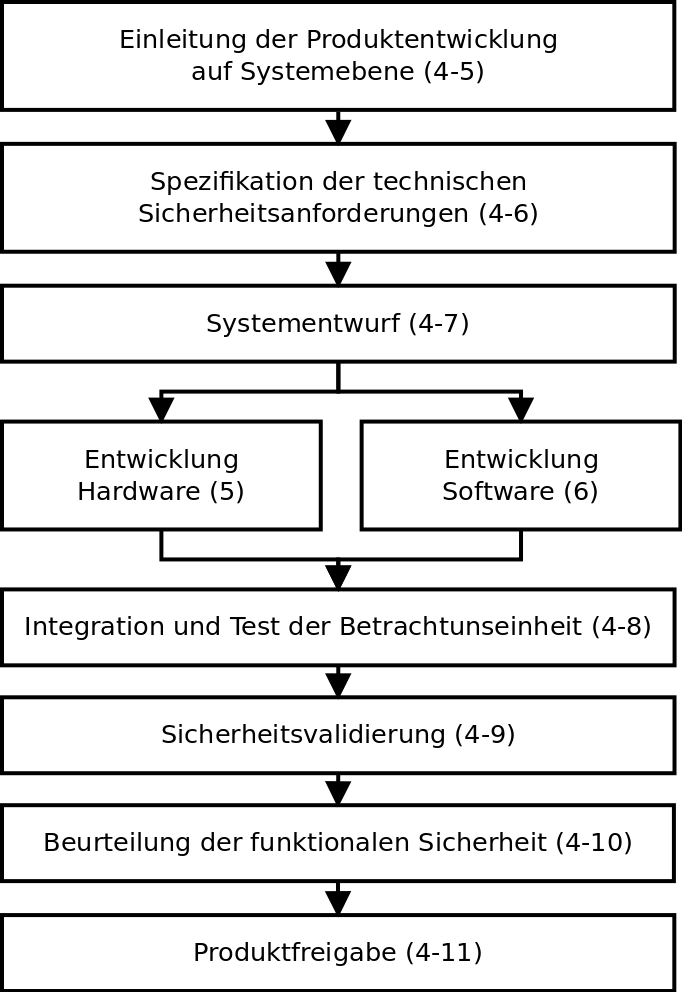
\includegraphics[width=4.5cm]{Abb_6_3}
\end{figure}

\end{frame}

\begin{frame}
\frametitle{Systemebene Methoden}

\begin{itemize}
    \item Entwurf der\dots
    \begin{itemize}
        \item \dots Hardware
        \item \dots Software
        \item \dots Testumgebung
        \item \dots Validierung
    \end{itemize}
    \item Spezifizierung der Metriken
    \item Einsatz von "`bewährten Architekturen"'
    \item Alle Schritte anhand des ASIL entwerfen und validieren
\end{itemize}

\end{frame}





\subsection{Hardware}
\begin{frame}
\frametitle{Hardware Überblick}

\begin{figure}
   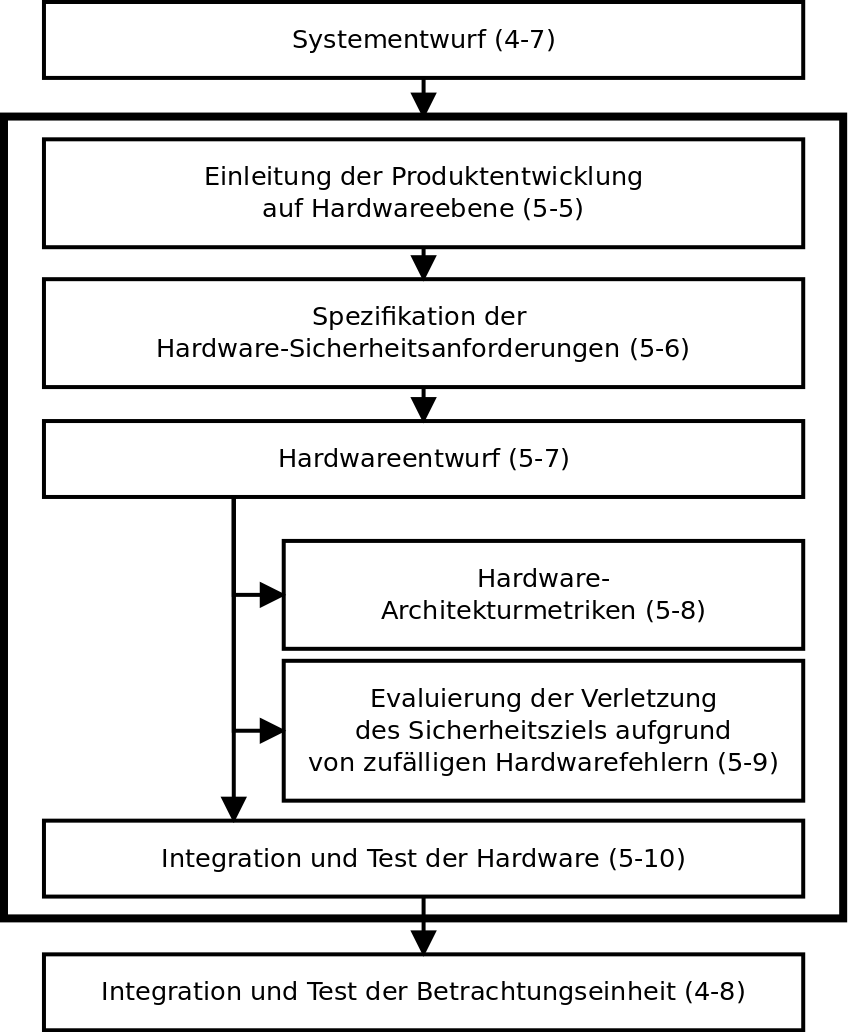
\includegraphics[width=5.4cm]{Abb_6_4}
\end{figure}

\end{frame}

\begin{frame}
\frametitle{Hardware Obergrenze Ausfallrate}

\begin{itemize}
    \item Obergrenze Ausfallrate
    \begin{itemize}
        \item Selbst ermittelbar oder
        \item Übernahme der Tabelle:
    \end{itemize}
\end{itemize}

\begin{center}
\begin{tabular}[h]{c r r c}
\toprule
ASIL & \multicolumn{3}{c}{Obergrenze für Ausfallrate}\\
\midrule
D & $ <10^{-8}/h $ & $ <10 $ FIT & Anforderung\\
C & $ <10^{-7}/h $ & $ <100 $ FIT   & Anforderung\\
B & $ <10^{-7}/h $ & $ <100 $ FIT   & Empfehlung\\
A & $ <10^{-6}/h $ & $ <1000 $ FIT   & Informativ\\
\bottomrule
\end{tabular}
\end{center}

\end{frame}

\begin{frame}
\frametitle{Hardware Fehlerarten}

\begin{itemize}
    \item Ungefährliche Fehler (safe fault; $ \lambda_S $)
    \item Einfachfehler (single point fault; $ \lambda_{SPF} $)
    \item Mehrfachfehler (multiple point fault; $ \lambda_{MPF} $)
    \item Schlafende Fehler (latent fault; $ L $)
    \item Erkannte oder wahrgenommene Fehler (detected or perceived fault; $ D, P $)
    \item Restfehler (residual fault; $ \lambda_{RF} $)
\end{itemize}

\end{frame}



\begin{frame}
\frametitle{Hardware Metriken}

\begin{itemize}
    \item Metriken geben Fehlertoleranz an
    \item Beschriebene Metriken:
    \item Single Point Fault Metric
    \begin{itemize}
        \item Betrachtet kritische Fehler ($ \lambda_{SPF}, \lambda_{RF} $)
        \item Beschreibt Risiko des Systems
    \end{itemize}
    \item Latent Fault Metric
    \begin{itemize}
        \item Betrachtet übrige Fehler ($ \lambda_{MPFD}, \lambda_{MPFP}, \lambda_{S} $)
        \item Beschreibt Verfügbarkeit des Systems
    \end{itemize}
\end{itemize}


\end{frame}




\subsection{Software}

\begin{frame}
\frametitle{Software Überblick}

\begin{figure}
   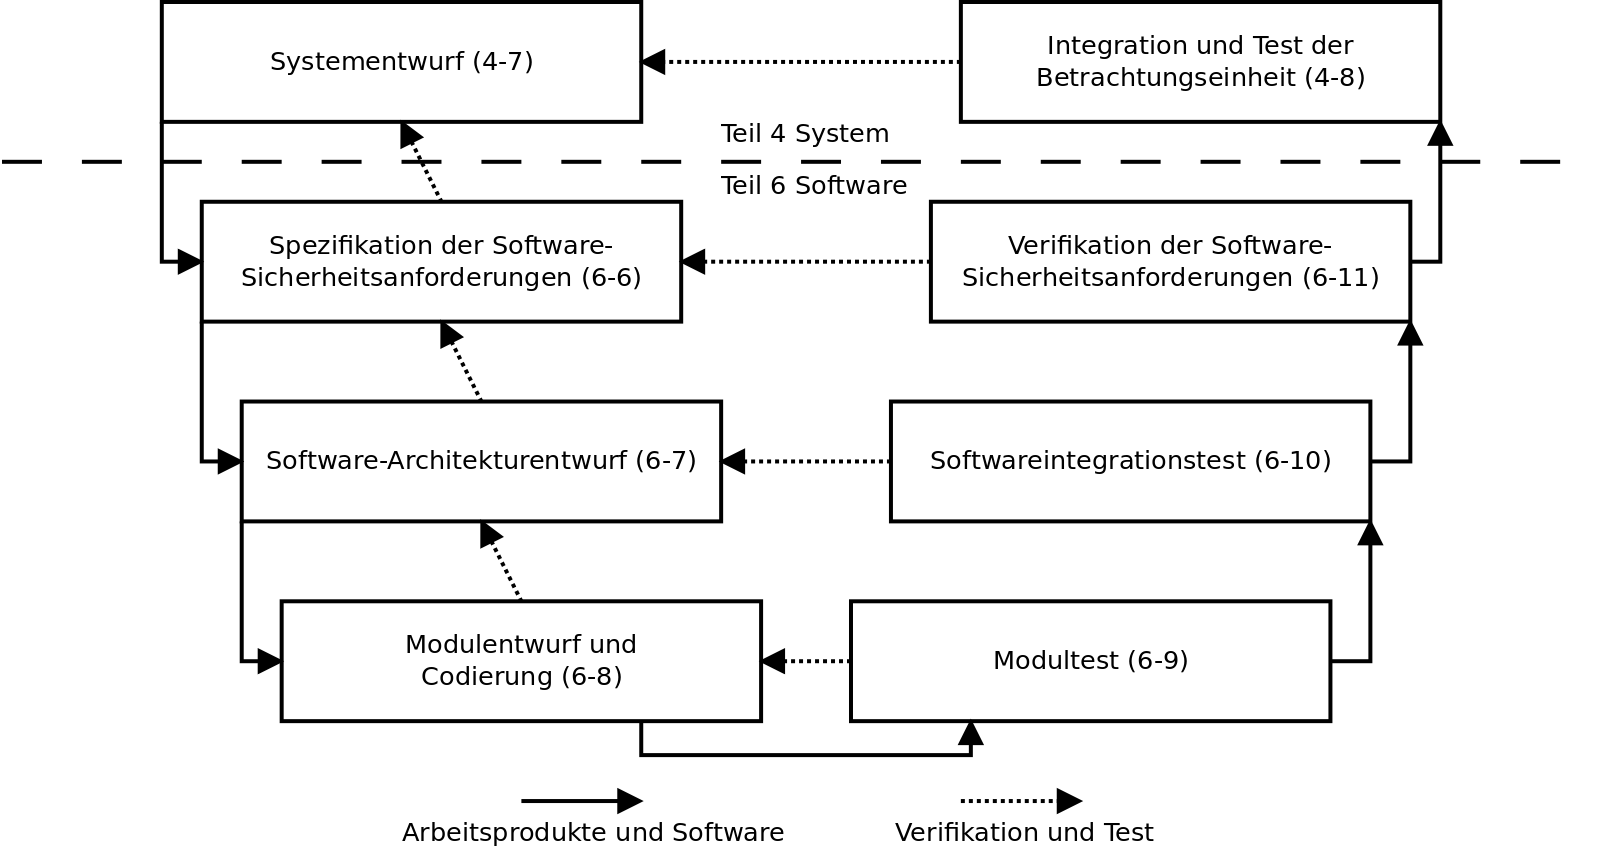
\includegraphics[width=11cm]{Abb_6_10}
\end{figure}

\end{frame}

\begin{frame}
\frametitle{Software Methoden}

\begin{itemize}
    \item ISO 26262 gibt grobe Tipps und Richtlinien
    \item Je ASIL unterschiedliche Anforderungen. Z.B.:
    \begin{itemize}
        \item ASIL B: Anweisungsüberdeckende Tests
        \item ASIL D: Tests nach MC/DC (DO-178B)
    \end{itemize}
    \item Allgemeine Einhaltung bestimmter Richtlinien (MISRA-C)
\end{itemize}

\end{frame}



%%%%%%%%%%%%%%%%%%%%%%%%%%%%%%%%%%%%%%%%%%%%%%%%%%%%%%%%%%%%%%%%%%%5
% Fazit
\section{Fazit}
\label{sec:Fazit}

\begin{frame}
\frametitle{Fazit}

\begin{itemize}
    \item Sammlung von Tipps und Best Practices
    \item Standard noch recht neu -> Wenig Informationen
    \item Rechtlich gefordert und damit zukunftsrelevant
\end{itemize}

\end{frame}








%%%%%%%%%%%%%%%%%%%%%%%%%%%%%%%%%%%%%%%%%%%%%%%%%%%%%%%%%%%%%%%%%%%5
% Literaturangaben
\appendix
\section*{Literatur}
\label{sec:Literatur}

\begin{frame}
\begin{thebibliography}{10}

\bibitem[1]{1} \textsc{Peter Löw, Roland Pabst, Erwin Petry}: {\em Funktionale Sicherheit in der Praxis.} dpunkt.verlag, 2010.

\end{thebibliography}
\end{frame}





















\end{document}










